\documentclass[aspectratio=169]{beamer}

\usetheme{Madrid}
\usecolortheme{default}

\usepackage[T1]{fontenc}
\usepackage[utf8]{inputenc}
\usepackage{listings}
\usepackage{xcolor}
\usepackage{booktabs}
\usepackage{tikz}
\usetikzlibrary{positioning, arrows.meta}

\title{AWK Interpreter \\ From Scratch in Three Languages}
\author{}
\date{}

\definecolor{codebg}{RGB}{245,245,245}
\definecolor{codegreen}{RGB}{34,139,34}
\definecolor{codeblue}{RGB}{0,0,180}

\lstset{
  basicstyle=\ttfamily\small,
  backgroundcolor=\color{codebg},
  keywordstyle=\color{codeblue},
  commentstyle=\color{codegreen},
  showstringspaces=false,
  frame=single,
  breaklines=true
}

\begin{document}

% ------------------------------------------------
\begin{frame}
  \titlepage
\end{frame}

% ------------------------------------------------
\begin{frame}[fragile]{What is AWK?}

A text-processing language from Bell Labs (1977).

\vspace{0.5em}

Programs are written as:

\[
\texttt{pattern \{ action \}}
\]

\vspace{1em}

\begin{lstlisting}[language=bash]
{ print $1, $3 }
/error/ { print NR, $0 }
BEGIN { sum = 0 }
END   { print sum }
\end{lstlisting}

\vspace{0.5em}

\begin{itemize}
  \item Reads from files or standard input
  \item Small, fast, dependency-free utility
  \item Excellent for structured text processing
\end{itemize}

\end{frame}

% ------------------------------------------------
\begin{frame}{Interpreter Pipeline}

\centering

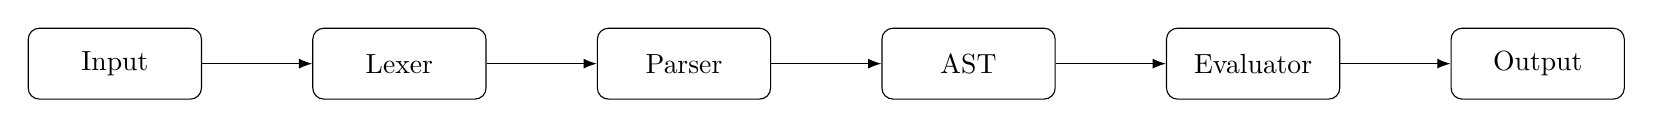
\begin{tikzpicture}[
  node distance=1.4cm,
  every node/.style={draw, rounded corners, minimum width=2.2cm, minimum height=0.9cm},
  >=Latex
]

\node (input) {Input};
\node[right=of input] (lexer) {Lexer};
\node[right=of lexer] (parser) {Parser};
\node[right=of parser] (ast) {AST};
\node[right=of ast] (eval) {Evaluator};
\node[right=of eval] (output) {Output};

\draw[->] (input) -- (lexer);
\draw[->] (lexer) -- (parser);
\draw[->] (parser) -- (ast);
\draw[->] (ast) -- (eval);
\draw[->] (eval) -- (output);

\end{tikzpicture}

\vspace{1.5em}

\begin{tabular}{ll}
\toprule
\textbf{Layer} & \textbf{Responsibility} \\
\midrule
Lexer & Source text to tokens \\
Parser & Tokens to syntax tree \\
AST & Node representation \\
Evaluator & Execute tree recursively \\
Builtins & AWK runtime functionality \\
\bottomrule
\end{tabular}

\end{frame}

% ------------------------------------------------
\begin{frame}{Project Goal}

Implement all major AWK features in:

\vspace{1em}

\begin{itemize}
  \item Rust
  \item Go
  \item Crystal
\end{itemize}

\vspace{1em}

\begin{table}
\small
\begin{tabular}{cl}
\toprule
\# & Feature \\
\midrule
1 & print with OFS/ORS \\
2 & Fields: \texttt{\$0}, \texttt{\$n}, NF, NR \\
3 & BEGIN/END and regex patterns \\
4 & Variables and arithmetic \\
5 & Field separators \\
6 & if/else \\
7 & Loops and control flow \\
8 & String functions \\
9 & Associative arrays \\
10 & printf formatting \\
\bottomrule
\end{tabular}
\end{table}

\end{frame}

% ------------------------------------------------
\begin{frame}{Languages and Timelines}

\begin{block}{Rust}
Primary implementation with all 10 features complete.
\end{block}

\begin{block}{Go}
Partial port implementing features 1--5.
\end{block}

\begin{block}{Crystal}
Full implementation with all 10 features complete.
\end{block}

\vspace{1em}

\begin{table}
\small
\begin{tabular}{ll}
\toprule
Date & Event \\
\midrule
\texttt{c1eef30} & Initial scaffold \\
\texttt{5a8a623} & Rust print support \\
\texttt{42bddb9} & Variables and arithmetic \\
\texttt{22ba7dd} & Loops and control flow \\
\texttt{ca53436} & Go port \\
\texttt{e6ddb9c} & Crystal full implementation \\
\bottomrule
\end{tabular}
\end{table}

\end{frame}

% ------------------------------------------------
\begin{frame}[fragile]{Rust Architecture}

\begin{lstlisting}
src/
├── main.rs       CLI + I/O
├── lexer.rs      Source → tokens
├── parser.rs     Tokens → AST
├── ast.rs        AST node types
├── value.rs      Dual-type values
├── builtins.rs   Builtins and runtime vars
└── interp.rs     Tree-walk evaluator
\end{lstlisting}

\vspace{0.8em}

\begin{itemize}
  \item Entire AST represented using enums
  \item Evaluation driven by pattern matching
  \item Recursive tree-walk interpreter
\end{itemize}

\end{frame}

% ------------------------------------------------
\begin{frame}[fragile]{Crystal Architecture}

\begin{lstlisting}
src/
├── awk.cr        CLI entry point
├── lexer.cr      Tokeniser
├── parser.cr     Recursive-descent parser
├── ast.cr        AST node classes
├── value.cr      AwkValue
├── builtins.cr   Runtime environment
└── interp.cr     Tree-walk evaluator
\end{lstlisting}

\vspace{0.8em}

\begin{itemize}
  \item Uses Crystal classes instead of enums
  \item Efficient output via String::Builder
  \item Explicit ControlFlow enum
\end{itemize}

\end{frame}

% ------------------------------------------------
\begin{frame}[fragile]{Key Design Decisions}

\textbf{Dual-Type Values}

\begin{lstlisting}
AwkValue holds either Float64 or String.
Arithmetic coerces to numbers.
Concatenation coerces to strings.
\end{lstlisting}

\vspace{1em}

\textbf{Control Flow Enum (Crystal)}

\begin{lstlisting}[language=C]
enum ControlFlow
  Normal | Break | Continue | Next | Exit
end
\end{lstlisting}

\vspace{1em}

\textbf{Execution Model}

\begin{itemize}
  \item No bytecode
  \item No JIT
  \item Pure recursive tree-walk evaluation
\end{itemize}

\end{frame}

% ------------------------------------------------
\begin{frame}{Bugs Found and Fixed}

\small

\begin{tabular}{p{0.25\linewidth} p{0.33\linewidth} p{0.25\linewidth}}
\toprule
\textbf{Bug} & \textbf{Cause} & \textbf{Fix} \\
\midrule
Variable assignment printed 0 & Assign node discarded & Added return \\
if/else crash & Parser skipped separators incorrectly & Skip semicolons \\
continue skipped updates & Wrong loop control handling & Run update expression \\
\$0 assignment failed & Empty field array unhandled & Initialize fields \\
Regex/division ambiguity & No lexer context & Inspect previous token \\
printf precision incorrect & Missing formatting support & Use sprintf \\
RLENGTH incorrect & Wrong constant value & Set to -1 \\
\bottomrule
\end{tabular}

\end{frame}

% ------------------------------------------------
\begin{frame}[fragile]{Testing Strategy}

\textbf{104 tests against system AWK}

\vspace{1em}

\begin{lstlisting}[language=bash]
1. Run system awk
2. Run custom interpreter
3. Compare outputs byte-for-byte
\end{lstlisting}

\vspace{1em}

\begin{block}{Result}
104 tests passed, 0 failed.
\end{block}

\vspace{0.5em}

This reference-based testing strategy caught every major semantic bug.

\end{frame}

% ------------------------------------------------
\begin{frame}{Feature Status}

\begin{table}
\small
\begin{tabular}{clccc}
\toprule
\# & Feature & Rust & Go & Crystal \\
\midrule
1 & print & ✅ & ✅ & ✅ \\
2 & Fields & ✅ & ✅ & ✅ \\
3 & BEGIN/END + regex & ✅ & ✅ & ✅ \\
4 & Variables/arithmetic & ✅ & ✅ & ✅ \\
5 & Field separator & ✅ & ✅ & ✅ \\
6 & if/else & ✅ & ❌ & ✅ \\
7 & Loops & ✅ & ❌ & ✅ \\
8 & String functions & ✅ & ❌ & ✅ \\
9 & Arrays & ✅ & ❌ & ✅ \\
10 & printf & ✅ & ❌ & ✅ \\
\bottomrule
\end{tabular}
\end{table}

\vspace{1em}

\begin{center}
Rust: 10/10 \qquad Go: 5/10 \qquad Crystal: 10/10
\end{center}

\end{frame}

% ------------------------------------------------
\begin{frame}[fragile]{Try It Yourself}

\begin{lstlisting}[language=bash]
cd crystal

# Build
crystal build src/awk.cr -o awk_crystal

# Run
./awk_crystal 'BEGIN{print "hello"}'

# Process fields
echo "hello world" | ./awk_crystal '{print $2}'

# CSV parsing
./awk_crystal -F, '{print $1, $3}' data.csv

# Test suite
./test.sh
\end{lstlisting}

\end{frame}

% ------------------------------------------------
\begin{frame}{Architecture Diagram}

\centering

\begin{tikzpicture}[
  node distance=1.5cm,
  every node/.style={draw, rounded corners, minimum width=2.8cm, minimum height=0.9cm},
  >=Latex
]

\node (source) {Source};
\node[below=of source] (lexer) {Lexer};
\node[below=of lexer] (parser) {Parser};
\node[below left=of parser] (builtins) {Builtins};
\node[below right=of parser] (ast) {AST};
\node[below=of parser, yshift=-2.2cm] (eval) {Evaluator};
\node[below=of eval] (stdout) {stdout};

\draw[->] (source) -- (lexer);
\draw[->] (lexer) -- (parser);
\draw[->] (parser) -- (ast);
\draw[->] (builtins) -- (eval);
\draw[->] (ast) -- (eval);
\draw[->] (eval) -- (stdout);

\end{tikzpicture}

\end{frame}

% ------------------------------------------------
\begin{frame}{Lessons Learned}

\begin{enumerate}
  \item AWK semantics are subtle and context-sensitive.

  \vspace{0.5em}

  \item Tree-walk interpreters are simple but capable.

  \vspace{0.5em}

  \item Porting across languages reveals hidden assumptions.

  \vspace{0.5em}

  \item Reference-based testing is extremely effective.
\end{enumerate}

\vspace{1.5em}

\begin{center}
\Large Questions?
\end{center}

\end{frame}

% ------------------------------------------------
\end{document}
